\section{二次惩罚法}
\label{sec:pm-quadratic}

把约束换成目标里的一笔费用之后，得到的解离原问题有多远，又要付出什么代价？

\paragraph{给违规计价}
可以把约束想成预算。硬约束相当于一分钱都不许超；惩罚的做法是允许超，但超得越多罚得越狠。费用要满足两点：可行时为零，不改变可行点上的目标；违规时为正，并且最好是光滑的，这样前面的无约束方法可以直接使用。

平方正好满足这两点。等式残差$h_j$偏离零时收$h_j^2$。不等式只有$g_i>0$时才算违规，所以先取正部
\[
 [a]_+=\max\{a,0\},
\]
再平方。把两类费用加到目标上，就得到下面的函数。

\begin{definition}[二次罚函数]
\label{def:pm-quadratic-penalty}
对问题~\eqref{eq:pm-problem}和\term{罚参数}（penalty parameter）$\rho>0$，\term{二次罚函数}（quadratic penalty function）是
\begin{equation}
 Q_\rho(\bm{x})=f(\bm{x})+\frac{\rho}{2}\Bigl(\sum_{i=1}^m[g_i(\bm{x})]_+^2+\sum_{j=1}^ph_j(\bm{x})^2\Bigr).
 \label{eq:pm-quadratic-penalty}
\end{equation}
依次近似最小化$Q_\rho$并逐步增大$\rho$的做法称为\term{二次惩罚法}（quadratic penalty method）。
\end{definition}

迭代点一般从可行集外面逼近，所以这类方法也叫外点法。正部的平方虽然含有$\max$，导数却是连续的：$\phi(a)=[a]_+^2$在$a<0$时为零，在$a>0$时为$a^2$，两边在$a=0$处的导数都是$0$，因此$\phi'(a)=2[a]_+$。由链式法则，当$f,g_i,h_j$都连续可微时，
\begin{equation}
 \nabla Q_\rho(\bm{x})=\nabla f(\bm{x})+\rho\sum_{i=1}^m[g_i(\bm{x})]_+\nabla g_i(\bm{x})+\rho\sum_{j=1}^ph_j(\bm{x})\nabla h_j(\bm{x}).
 \label{eq:pm-quadratic-gradient}
\end{equation}
要注意$\phi''$在$a=0$处跳跃，所以有不等式约束时$Q_\rho$一般只是一阶连续可微，二阶导数在约束边界上不连续。

\begin{example}[一维例的二次罚]
\label{ex:pm-quadratic-one-dim}
式~\eqref{eq:pm-one-dim}的$g(x)=1-x$，罚函数是
\[
 Q_\rho(x)=x+\frac{\rho}{2}[1-x]_+^2 .
\]
当$x\geq1$时，$Q_\rho'(x)=1>0$，这部分没有驻点。当$x<1$时，
\[
 Q_\rho'(x)=1-\rho(1-x).
\]
令其为零，解出
\[
 x_\rho=1-\frac1\rho .
\]
$Q_\rho$是凸函数，所以这个驻点是全局最小点。它落在可行集外，违规量恰好是$1/\rho$。
\end{example}

图~\ref{fig:pm-quad-1d}画出$\rho=1,2,5$时的$Q_\rho$。绿点随$\rho$增大向右移动，始终停在竖线左边，不可行。绿点的高度是$Q_\rho(x_\rho)=1-1/(2\rho)$，比原问题的最优值$1$低。可见罚目标的值既不是原目标，也不是最优值的上界，降低罚目标和满足原约束是两件要分别检查的事。

\begin{BookInlineFigure}
  \centering
  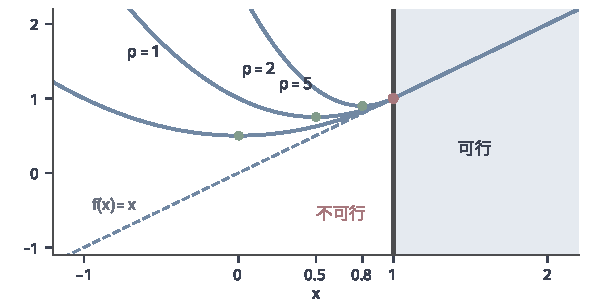
\includegraphics[width=100mm]{figures/05-optimization/06-constrained-optimization/matplotlib/pm-quad-1d/figure.pdf}
  \caption{一维例的二次罚函数，$\rho=1,2,5$。蓝色实线是$Q_\rho$，蓝色虚线是原目标$f(x)=x$，浅蓝区域是可行集，深灰竖线是约束边界。绿点是$Q_\rho$的最小点$x_\rho=1-1/\rho$，红点是原问题的解。有限的$\rho$下最小点总在边界左侧。}
  \label{fig:pm-quad-1d}
\end{BookInlineFigure}

\paragraph{力的平衡}
为什么有限的$\rho$总留下违规？把驻点方程$\rho(1-x_\rho)=1$读成力的平衡。目标以大小为$1$的力把$x$往左拉，罚项像一根劲度为$\rho$的弹簧往右推。弹簧必须被拉长才有力，要平衡$1$的力就得拉长$1/\rho$。弹簧越硬，拉长越少，但只要力不为零，拉长量就不为零。

这个力的大小$\rho(1-x_\rho)=1$恰好是最优乘子$\lambda^\star=1$。第~\ref{chap:constrained-optimality}章说过，乘子度量约束对目标的反作用力。这里违规量乘罚参数等于乘子，并不是一维例的巧合，后面会看到它的一般形式。类比也有失效的地方：真实的弹簧两边都有力，而不等式的罚项只在违规一侧起作用。

\begin{example}[二元例的二次罚]
\label{ex:pm-quadratic-running}
对式~\eqref{eq:pm-running}，罚函数是
\[
 Q_\rho(\bm{x})=\frac12x_1^2+\frac32x_2^2+\frac\rho2(x_1+x_2-4)^2 .
\]
令梯度为零，得到两个线性方程：
\[
 (1+\rho)x_1+\rho x_2=4\rho,\qquad \rho x_1+(3+\rho)x_2=4\rho .
\]
两式相减得$x_1=3x_2$。代回第二式，解出
\begin{equation}
 x_2(\rho)=\frac{4\rho}{3+4\rho},\qquad x_1(\rho)=\frac{12\rho}{3+4\rho}.
 \label{eq:pm-running-penalty-solution}
\end{equation}
由此算出约束残差
\begin{equation}
 h(\bm{x}(\rho))=-\frac{12}{3+4\rho}.
 \label{eq:pm-running-penalty-residual}
\end{equation}
它在$\rho\to\infty$时以$1/\rho$的速度趋于零，而$\rho h(\bm{x}(\rho))$趋于$-3$，正是$\nu^\star$。
\end{example}

图~\ref{fig:pm-penalty-contours}是同一个例子的二维图景。深灰直线是约束，绿点是$Q_\rho$的最小点。$\rho$增大时等高线沿直线方向被拉长，绿点向红点靠近。

\begin{BookInlineFigure}
  \centering
  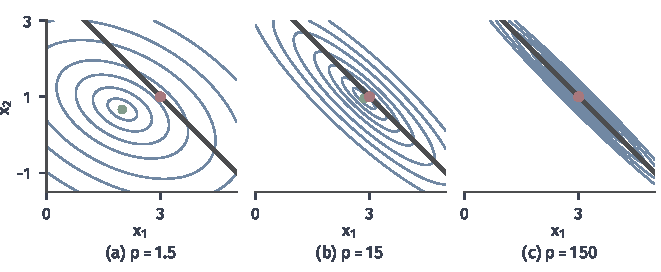
\includegraphics[width=112mm]{figures/05-optimization/06-constrained-optimization/matplotlib/pm-penalty-contours/figure.pdf}
  \caption{二元例中$Q_\rho$的等高线（蓝）。深灰直线是约束$x_1+x_2=4$，绿点是$Q_\rho$的最小点，红点是原问题的解$(3,1)$。$\rho$增大时最小点靠近解，等高线同时变成贴着约束的狭长椭圆。}
  \label{fig:pm-penalty-contours}
\end{BookInlineFigure}

\subsection{罚参数的更新}
\label{sec:pm-rho-update}

\paragraph{主要思想}
式~\eqref{eq:pm-running-penalty-residual}提示一开始就把$\rho$取得很大，一次解完。这样做的问题在于，$\rho$大的罚问题很难解，本节后面会算出来。如果从不好的初值开始，内层算法可能花大量步数才能进入解的附近。

合理的做法是沿着$\rho$的路径走。先取较小的$\rho$，解一个容易的问题；再放大$\rho$，以上一轮的解作为初值。$\rho$只放大有限倍时，新解离旧解不远，这叫\term{热启动}（warm start）。外层循环的结构如图~\ref{fig:pm-outer-loop}所示。

\begin{BookInlineFigure}
  \centering
  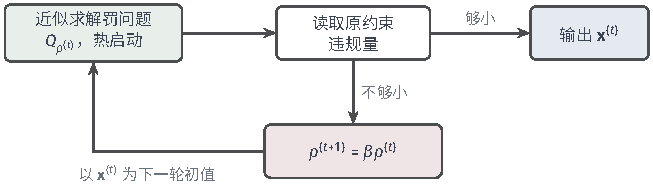
\includegraphics[width=110mm]{figures/05-optimization/06-constrained-optimization/tikz/pm-outer-loop/figure.pdf}
  \caption{二次惩罚法的外层循环。绿框是内层的无约束求解，蓝框是输出；判断依据是原约束的违规量，而不是罚目标的大小。只有违规量不够小时才放大罚参数（红框）。}
  \label{fig:pm-outer-loop}
\end{BookInlineFigure}

这里有两个容差，分工不同。内层容差$\omega^{(t)}$控制$\lVert\nabla Q_{\rho^{(t)}}(\bm{x}^{(t)})\rVert_2$，说明这一轮的罚问题解得多准。外层容差$\varepsilon$控制原约束的违规量，说明原问题的可行性够不够。内层梯度很小，只说明罚问题解好了，不能据此宣布原问题已解。

放大规则取固定倍数$\beta>1$，并记录乘子估计：
\begin{equation}
 \rho^{(t+1)}=\beta\rho^{(t)},\qquad
 \nu_j^{(t)}=\rho^{(t)}h_j(\bm{x}^{(t)}),\qquad
 \lambda_i^{(t)}=\rho^{(t)}[g_i(\bm{x}^{(t)})]_+ .
 \label{eq:pm-penalty-update}
\end{equation}
这组估计的来历可以从式~\eqref{eq:pm-quadratic-gradient}读出：把它们代入，$\nabla Q_{\rho}$恰好是Lagrange函数对$\bm{x}$的梯度。内层求解到梯度为零，就等于Lagrange驻定条件在这组估计下成立。

\paragraph{计算过程}
以二元例为例，内层用步长为$1/L$的梯度法，其中$L$是$\nabla^2Q_\rho$的最大特征值。

\needspace{6\baselineskip}
\paragraph{变量}
\begin{itemize}
 \item $\bm{x}^{(t)}\in\mathbb{R}^n$：第$t$轮罚问题的近似解。例中$n=2$。
 \item $\rho^{(t)}>0$：罚参数，放大倍数为$\beta>1$。
 \item $\varepsilon$、$\omega^{(t)}$：外层违规容差、内层梯度容差。
\end{itemize}

\paragraph{初始化}
取初值$\bm{x}^{(-1)}$、$\rho^{(0)}>0$和$\beta$。例中$\bm{x}^{(-1)}=(0,0)$，$\rho^{(0)}=1.5$，$\beta=10$，外层容差$\varepsilon=0.05$，内层容差取常数$\omega^{(t)}=10^{-3}$。

\needspace{6\baselineskip}
\paragraph{每轮更新}
\begin{enumerate}
 \item 从$\bm{x}^{(t-1)}$出发近似最小化$Q_{\rho^{(t)}}$，直到梯度范数不超过$\omega^{(t)}$。例中第一轮用了$21$个梯度步，结果接近式~\eqref{eq:pm-running-penalty-solution}的精确解，以下数值用精确解给出：
 \[
  \bm{x}^{(0)}=\Bigl(2,\ \frac23\Bigr).
 \]

 \item 计算违规量。例中第一轮
 \[
  h(\bm{x}^{(0)})=-\frac43,\qquad \lvert h(\bm{x}^{(0)})\rvert>\varepsilon .
 \]
 \item 若违规量不超过$\varepsilon$，结束；否则由式~\eqref{eq:pm-penalty-update}放大罚参数并记录乘子估计。例中第一轮
 \[
  \rho^{(1)}=15,\qquad \nu^{(0)}=1.5\times\Bigl(-\frac43\Bigr)=-2 .
 \]
\end{enumerate}
例中第二轮从$\bm{x}^{(0)}$热启动，用了$107$个梯度步，得到
\[
 \bm{x}^{(1)}=\Bigl(\frac{20}{7},\ \frac{20}{21}\Bigr),\qquad
 h(\bm{x}^{(1)})=-\frac{4}{21}\approx-0.190 .
\]
乘子估计是$\nu^{(1)}=-\tfrac{20}{7}\approx-2.857$。
违规量仍大于$0.05$，于是$\rho^{(2)}=150$。第三轮用了$725$个梯度步，得到
\[
 \bm{x}^{(2)}=\Bigl(\frac{200}{67},\ \frac{200}{201}\Bigr),\qquad
 h(\bm{x}^{(2)})=-\frac{4}{201}\approx-0.020 .
\]
乘子估计是$\nu^{(2)}=-\tfrac{200}{67}\approx-2.985$。

结束条件是违规量不超过$\varepsilon$，例中在第三轮满足。最终得到$\bm{x}^{(2)}\approx(2.985,0.995)$，目标值$f(\bm{x}^{(2)})\approx5.940$，略低于$f^\star=6$，这是因为点还不可行。三轮的梯度步数依次是$21$、$107$、$725$，几乎全部花在最后一轮上。步数为什么增长这么快，正是下一小节要回答的。

\subsection{极限与病态}
\label{sec:pm-limit}

这一小节回答两个问题：$\rho\to\infty$时迭代点到底趋于什么，以及这条路有多贵。

\paragraph{全局解的极限}
先看最理想的情形，每一轮都得到罚问题的全局最小点。此时可以把罚目标与任意一个可行点比较，这个比较给出全部结论。

\begin{theorem}[二次惩罚法的全局极限]
\label{thm:pm-quadratic-limit}
设$f$、$g_i$、$h_j$在$\mathbb{R}^n$上连续，可行集$\bm{C}$非空，且$f$在$\mathbb{R}^n$上有下界$f_{\mathrm{low}}$。设$\rho^{(t)}\to\infty$，每个$\bm{x}^{(t)}$都是$Q_{\rho^{(t)}}$的全局最小点。记
\begin{equation}
 v(\bm{x})=\sum_{i=1}^m[g_i(\bm{x})]_+^2+\sum_{j=1}^ph_j(\bm{x})^2 .
 \label{eq:pm-violation-square}
\end{equation}
则对任一可行点$\bar{\bm{x}}\in\bm{C}$，有
\begin{equation}
 v(\bm{x}^{(t)})\leq\frac{2\bigl(f(\bar{\bm{x}})-f_{\mathrm{low}}\bigr)}{\rho^{(t)}},
 \label{eq:pm-quadratic-violation-bound}
\end{equation}
并且$\{\bm{x}^{(t)}\}$的每个聚点都是原问题的全局最优解。
\end{theorem}

\begin{proof}
可行点上罚项为零，$Q_{\rho^{(t)}}(\bar{\bm{x}})=f(\bar{\bm{x}})$。$\bm{x}^{(t)}$是全局最小点，所以
\[
 f(\bm{x}^{(t)})+\frac{\rho^{(t)}}{2}v(\bm{x}^{(t)})\leq f(\bar{\bm{x}}).
\]
左边第一项用$f_{\mathrm{low}}$放缩，整理即得式~\eqref{eq:pm-quadratic-violation-bound}。

设$\hat{\bm{x}}$是一个聚点，子列收敛到它。$v$连续，而式~\eqref{eq:pm-quadratic-violation-bound}的右边趋于零，所以$v(\hat{\bm{x}})=0$，即$\hat{\bm{x}}$可行。

上面的不等式中罚项非负，去掉后得到
\[
 f(\bm{x}^{(t)})\leq f(\bar{\bm{x}}).
\]
沿子列取极限，由$f$连续得$f(\hat{\bm{x}})\leq f(\bar{\bm{x}})$。$\bar{\bm{x}}$是任取的可行点，所以$\hat{\bm{x}}$全局最优。
\end{proof}

各条件的作用分得很清楚。可行集非空提供了比较点$\bar{\bm{x}}$。下界把违规量和$\rho$联系起来。连续性保证极限可行，并让目标比较传到极限。“全局最小点”是证明的关键一步，局部解不能和远处的可行点比较。定理也不保证聚点存在：序列可能跑向无穷远，要排除这种情形，还需要类似水平集有界的条件。

去掉下界会怎样？考虑$\min x^3$，$x\geq0$，解是$x^\star=0$。罚函数在$x<0$时等于$x^3+\tfrac\rho2x^2$，$x\to-\infty$时趋于$-\infty$，所以对任何$\rho$都没有全局最小点。图~\ref{fig:pm-failures}(a)画出了这种情形：$x=0$附近有一个局部的谷，越过左侧的小山就一路下降。原问题完全正常，罚问题却无下界。

\paragraph{近似解的极限}
实际算法只能给出梯度小的点，通常连局部最小都不能保证。这时比较可行点的论证失效，能说的话变少，并且要多加条件。下面只写等式约束，记$\bm{h}(\bm{x})=(h_1(\bm{x}),\ldots,h_p(\bm{x}))$，$\bm{J}(\bm{x})\in\mathbb{R}^{p\times n}$是它的Jacobian矩阵。

\begin{theorem}[近似驻点的极限]
\label{thm:pm-quadratic-approximate}
设$f,h_j$连续可微，$\rho^{(t)}\to\infty$，并且
\begin{equation}
 \lVert\nabla Q_{\rho^{(t)}}(\bm{x}^{(t)})\rVert_2\leq\omega^{(t)}\to0 .
 \label{eq:pm-inner-accuracy}
\end{equation}
设$\hat{\bm{x}}$是$\{\bm{x}^{(t)}\}$的聚点，则$\hat{\bm{x}}$是$\tfrac12\lVert\bm{h}\rVert_2^2$的驻点。若进一步$\hat{\bm{x}}$可行且$\bm{J}(\hat{\bm{x}})$行满秩，则沿收敛到$\hat{\bm{x}}$的子列有
\begin{equation}
 \rho^{(t)}\bm{h}(\bm{x}^{(t)})\to\hat{\bm{\nu}},\qquad
 \nabla f(\hat{\bm{x}})+\bm{J}(\hat{\bm{x}})^\top\hat{\bm{\nu}}=\bm{0},
 \label{eq:pm-multiplier-limit}
\end{equation}
即$(\hat{\bm{x}},\hat{\bm{\nu}})$满足KKT条件。
\end{theorem}

\begin{proof}
记$\bm{e}^{(t)}=\nabla Q_{\rho^{(t)}}(\bm{x}^{(t)})$，$\bm{e}^{(t)}\to\bm{0}$。为简化写法，下面的量都沿子列取，并省略$\bm{x}^{(t)}$的自变量。由梯度公式，
\[
 \nabla f+\rho^{(t)}\bm{J}^\top\bm{h}=\bm{e}^{(t)}.
\]
两边除以$\rho^{(t)}$，得到
\[
 \bm{J}^\top\bm{h}=\frac{\bm{e}^{(t)}-\nabla f}{\rho^{(t)}}.
\]
右边的分子有界，分母趋于无穷，取极限得
\[
 \bm{J}(\hat{\bm{x}})^\top\bm{h}(\hat{\bm{x}})=\bm{0}.
\]
左边正是$\tfrac12\lVert\bm{h}\rVert_2^2$的梯度，第一个结论成立。

再设$\hat{\bm{x}}$可行且$\bm{J}(\hat{\bm{x}})$行满秩。$\bm{J}\bm{J}^\top$连续且极限可逆，所以$t$足够大时可逆。用$\bm{J}$左乘第一个等式再求逆，解出
\[
 \rho^{(t)}\bm{h}=(\bm{J}\bm{J}^\top)^{-1}\bm{J}\bigl(\bm{e}^{(t)}-\nabla f\bigr).
\]
右边收敛，记极限为$\hat{\bm{\nu}}$。把$\rho^{(t)}\bm{h}\to\hat{\bm{\nu}}$代回第一个等式取极限，即得式~\eqref{eq:pm-multiplier-limit}。
\end{proof}

这个定理有两点值得注意。第一，$\hat{\bm{x}}$完全可能不可行，它只是约束残差平方的驻点。第二，定理的结论停在KKT点，和全局最优还差得远。

下面的例子显示第一点确实会发生。取
\[
 \min_x\ \frac12x^2\qquad\text{s.t.}\qquad h(x)=x^3-3x+3=0 .
\]
三次方程只有一个实根$x^\star\approx-2.104$，这也是唯一的可行点。$h$在$x=1$处有局部极小值$h(1)=1$，所以$\tfrac12h^2$在这里有一个不可行的局部谷。图~\ref{fig:pm-failures}(b)中绿点是$Q_3$在这个谷里的局部最小点。

取$\rho=10$和$\rho=100$，用二分法解$Q_\rho'(x)=0$，得到谷中的驻点分别是
\[
 x_{10}\approx0.9835,\qquad x_{100}\approx0.9983 .
\]
这两个点上$Q_\rho$的梯度为零，$h$却约等于$1$。放大$\rho$只会让点更靠近$x=1$，乘子估计$\rho h$随之发散。乘子估计发散正是不可行极限的常见信号。

\begin{BookInlineFigure}
  \centering
  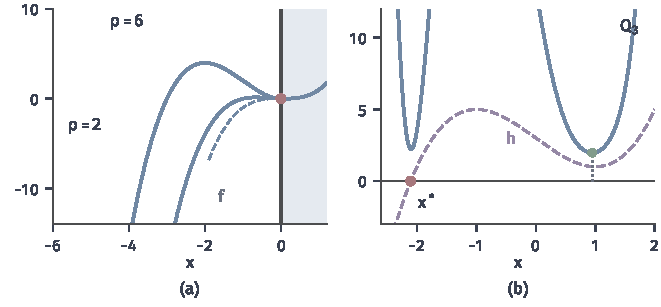
\includegraphics[width=112mm]{figures/05-optimization/06-constrained-optimization/matplotlib/pm-failures/figure.pdf}
  \caption{二次惩罚法的两种失败。(a)$\min x^3$，$x\geq0$：蓝色实线是$\rho=2,6$的罚函数，虚线是$f$的一段，浅蓝区域可行，红点是解；$x\to-\infty$时罚函数无下界。(b)$\min\tfrac12x^2$，$h(x)=x^3-3x+3=0$：紫色虚线是$h$，蓝线是$Q_3$，红点是唯一的可行点，绿点是不可行的局部最小点。}
  \label{fig:pm-failures}
\end{BookInlineFigure}

\paragraph{法向曲率的增长}
剩下的问题是代价。对等式约束的罚函数求二阶导，得到
\begin{equation}
 \nabla^2Q_\rho=\nabla^2f+\rho\sum_{j=1}^ph_j\nabla^2h_j+\rho\bm{J}^\top\bm{J}.
 \label{eq:pm-penalty-hessian}
\end{equation}
由定理~\ref{thm:pm-quadratic-approximate}，$\rho h_j$在解附近接近有限的乘子，前两项之和接近Lagrange函数的Hessian，大小不随$\rho$增长。第三项却正比于$\rho$，它只在$\bm{J}$的行空间里起作用，也就是约束的法方向上。

线性约束的二次目标可以把这件事算清楚。设目标和约束分别是
\[
 f(\bm{x})=\frac12\bm{x}^\top\bm{G}\bm{x}-\bm{d}^\top\bm{x},\qquad\bm{h}(\bm{x})=\bm{A}\bm{x}-\bm{b},
\]
其中$\bm{A}\in\mathbb{R}^{p\times n}$，$p<n$，$\bm{G}$半正定。此时$\nabla^2Q_\rho=\bm{G}+\rho\bm{A}^\top\bm{A}$不依赖$\bm{x}$。

\begin{lemma}[罚函数Hessian的条件数]
\label{lem:pm-penalty-condition}
设$\bm{A}\neq\bm{0}$，$\bm{Z}$的列是$\operatorname{null}(\bm{A})$的一组标准正交基，矩阵$\bm{Z}^\top\bm{G}\bm{Z}$正定，$\sigma_{\max}(\bm{A})$是$\bm{A}$的最大奇异值。记$\bm{H}_\rho=\bm{G}+\rho\bm{A}^\top\bm{A}$。当$\bm{H}_\rho$正定时，有
\begin{equation}
 \lambda_{\max}(\bm{H}_\rho)\geq\rho\,\sigma_{\max}(\bm{A})^2,\qquad
 \lambda_{\min}(\bm{H}_\rho)\leq\lambda_{\min}(\bm{Z}^\top\bm{G}\bm{Z}),
 \label{eq:pm-penalty-eigen-bounds}
\end{equation}
于是条件数满足
\begin{equation}
 \kappa(\bm{H}_\rho)\geq\frac{\rho\,\sigma_{\max}(\bm{A})^2}{\lambda_{\min}(\bm{Z}^\top\bm{G}\bm{Z})}.
 \label{eq:pm-penalty-condition}
\end{equation}
\end{lemma}

\begin{proof}
两个界都来自Rayleigh商。设$\bm{u}$是$\bm{A}$对应最大奇异值的单位右奇异向量。由$\bm{G}$半正定，
\[
 \lambda_{\max}(\bm{H}_\rho)\geq\bm{u}^\top\bm{H}_\rho\bm{u}\geq\rho\lVert\bm{A}\bm{u}\rVert_2^2=\rho\,\sigma_{\max}(\bm{A})^2 .
\]
再取单位向量$\bm{w}$，使它达到$\bm{Z}^\top\bm{G}\bm{Z}$的最小特征值，并令$\bm{y}=\bm{Z}\bm{w}$。$\bm{y}$是单位向量且$\bm{A}\bm{y}=\bm{0}$，所以罚项消失：
\[
 \lambda_{\min}(\bm{H}_\rho)\leq\bm{y}^\top\bm{H}_\rho\bm{y}=\bm{w}^\top\bm{Z}^\top\bm{G}\bm{Z}\bm{w}=\lambda_{\min}(\bm{Z}^\top\bm{G}\bm{Z}).
\]
两式相除，即得式~\eqref{eq:pm-penalty-condition}。
\end{proof}

几何上看，$\bm{H}_\rho$把空间分成两部分：沿约束的切方向，曲率不受$\rho$影响；沿法方向，曲率约正比于$\rho$。这就是图~\ref{fig:pm-penalty-contours}里等高线越来越狭长的原因。

二元例中$\bm{G}=\operatorname{diag}(1,3)$，$\bm{A}=(1,1)$，$\sigma_{\max}(\bm{A})^2=2$。切方向是单位向量$(1,-1)/\sqrt2$，切向曲率是
\[
 \bm{Z}^\top\bm{G}\bm{Z}=\frac{1+3}{2}=2 .
\]
下表给出$\bm{H}_\rho$的实际特征值，最小特征值逐渐接近切向曲率$2$，最大特征值约等于$2\rho$。

\begin{BookInlineTable}
  \centering
  \begin{tabular}{@{}rrrr@{}}
    \toprule
    $\rho$ & $\lambda_{\min}$ & $\lambda_{\max}$ & $\kappa$\\
    \midrule
    $1.5$ & $1.697$ & $5.303$ & $3.1$\\
    $15$ & $1.967$ & $32.03$ & $16.3$\\
    $150$ & $1.997$ & $302.0$ & $151.3$\\
    $1500$ & $2.000$ & $3002$ & $1501$\\
    \bottomrule
  \end{tabular}
  \caption{二元例中罚函数Hessian的特征值与条件数。}
  \label{tab:pm-penalty-condition}
\end{BookInlineTable}

图~\ref{fig:pm-conditioning}把精度和代价放在一起。(a)是违规量，$\rho$放大十倍，违规量缩小十倍。(b)是条件数和梯度步数，$\rho$放大十倍，条件数也放大十倍，每轮的梯度步数增长的倍数相近。

\begin{BookInlineFigure}
  \centering
  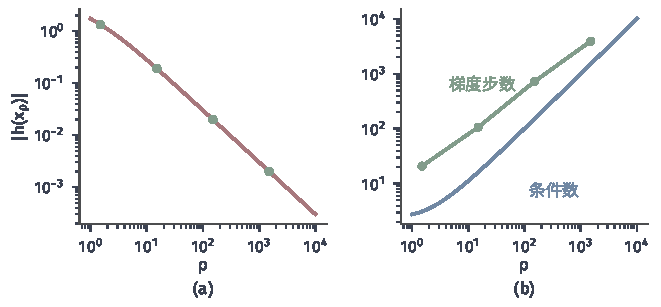
\includegraphics[width=112mm]{figures/05-optimization/06-constrained-optimization/matplotlib/pm-conditioning/figure.pdf}
  \caption{二元例中罚参数的收益与代价，双对数坐标。(a)精确罚解的违规量$12/(3+4\rho)$，绿点是$\rho=1.5,15,150,1500$。(b)蓝线是$\nabla^2Q_\rho$的条件数，绿线是热启动的梯度法（步长$1/L$，梯度容差$10^{-3}$）在各轮用的步数。}
  \label{fig:pm-conditioning}
\end{BookInlineFigure}

梯度法的困难可以直接看到。图~\ref{fig:pm-gd-penalty}从同一点出发各走$25$步。$\rho=1.5$时点很快到达最小点附近；$\rho=15$时第一步几乎只修正法向，点落到直线旁边，然后沿狭长山谷缓慢爬行，$25$步还没有走到。步长受最大曲率限制，只能取$1/L\approx1/(2\rho)$，切方向每步却只能修正很小一部分。

\begin{BookInlineFigure}
  \centering
  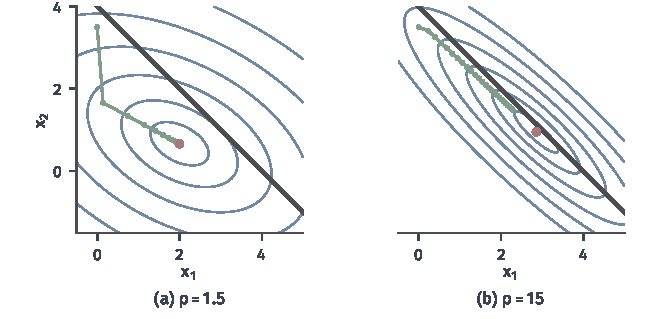
\includegraphics[width=112mm]{figures/05-optimization/06-constrained-optimization/matplotlib/pm-gd-penalty/figure.pdf}
  \caption{梯度法在$Q_\rho$上的路径，起点$(0,3.5)$，步长$1/L$，共$25$步。蓝线是$Q_\rho$的等高线，深灰直线是约束，绿色折线是迭代路径，红点是$Q_\rho$的最小点。(a)$\rho=1.5$，几步后接近最小点。(b)$\rho=15$，先快速到达山谷，再沿谷底缓慢前进。}
  \label{fig:pm-gd-penalty}
\end{BookInlineFigure}

病态是否致命，取决于内层用什么方法。Newton法不怕目标的简单伸缩，但线性方程组$\bm{H}_\rho\bm{d}=-\nabla Q_\rho$的系数矩阵本身条件数很差。引入$\bm{w}=\rho\bm{A}\bm{d}$，可以把它等价地写成
\begin{equation}
 \begin{pmatrix}\bm{G}&\bm{A}^\top\\\bm{A}&-\rho^{-1}\bm{I}\end{pmatrix}
 \begin{pmatrix}\bm{d}\\\bm{w}\end{pmatrix}
 =\begin{pmatrix}-\nabla Q_\rho\\\bm{0}\end{pmatrix}.
 \label{eq:pm-penalty-augmented-system}
\end{equation}
$\rho\to\infty$时这个系统趋于一个不含大数的KKT矩阵，数值上稳定得多。这个变换改善的是线性代数的数值误差，并不减少外层要解的问题个数。一阶方法没有这种办法。第~\ref{sec:pm-alm}节要给出另一条出路：不把$\rho$推向无穷。
